Sau quá trình thực hiện luận văn, bằng cách sử dụng những công nghệ và kiên thức được đưa ra trong các phần trước, nhóm đã hoàn thành một Hệ thống quản lí vải nhuộm tương đối hoàn chỉnh.\par

Tài liệu về các API nhóm đã hiện thực và sử dụng trong hệ thống: \href{http://bit.ly/api-lvtn-202}{API Documentation [http://bit.ly/api-lvtn-202]}

Phần sau đây nhóm sẽ trình bày về giao diện ứng dụng mà nhóm hiện thực, cũng như hướng giải quyết các vấn đề gặp phải trong khi hiện thực.

%%%%%%%%%%%%%%%%%%%%%%%%
\textbf{Trang đăng nhập}

Sau khi được Quản trị hệ thống cung cấp tài khoản, người dùng có thể đăng nhập vào hệ thống ở trang Đăng nhập [\ref{result_dang_nhap}]. Sau khi đăng nhập thành công, tài khoản này sẽ được server cung cấp một token để thực hiện các yêu cầu API xuyên suốt trong quá trình xử dụng ứng dụng. Token sẽ hết hạn nếu như sau 30 phút không có bất cứ yêu cầu nào lên server, khi này người dùng cần đăng nhập lại để tiếp tục sử dụng.\par
Token được lưu trữ ở Local Storage, việc lưu trữ nằm nhằm mục đích khi người dùng tải lại trang, tất cả state của hệ thống sẽ bị xóa, khi này sẽ lấy token đã lưu để lấy lại thông tin mà không yêu cầu người dùng phải đăng nhập lại.
\begin{figure}[H]
    \begin{center}
        \frame{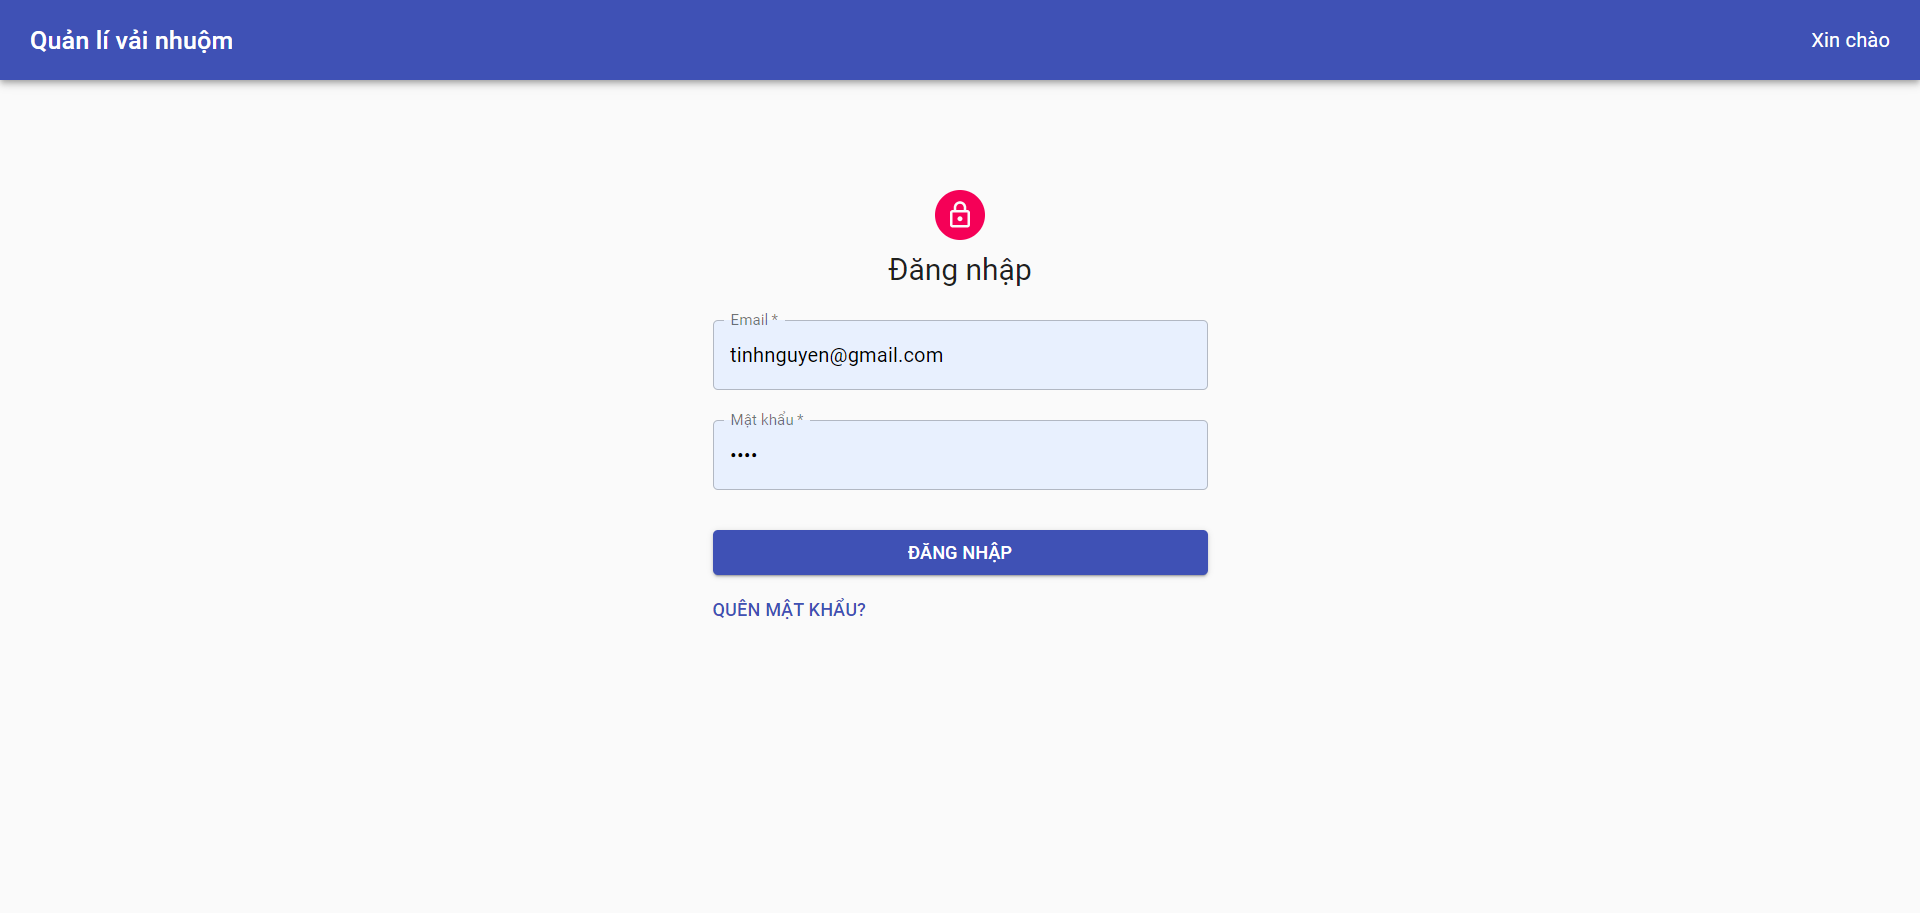
\includegraphics[width=12cm]{Image/result/dang_nhap.png}}
        \caption{Giao diện trang đăng nhập}
        \label{result_dang_nhap}
    \end{center}
\end{figure}



% %%%%%%%%%%%%%%%%%%%%%%%%
% \textbf{}

% \begin{figure}[H]
%     \begin{center}
%         \frame{\includegraphics[width=12cm]{Image/result/}}
%         \caption{}
%         \label{result_}
%     \end{center}
% \end{figure}